\documentclass[11pt,a4paper]{jsarticle}

\usepackage[dvipdfmx]{graphicx}
\usepackage{fancyvrb}
\usepackage{ascmac}
\usepackage{mediabb}

\begin{document}

\title{並列分散処理 最終報告書}
\author{135772H 上原可意\\145758G 森井大介\\155702F 大城由也\\155728K 津嘉山遼\\155737J 松本直也\\}
\date{2017/8/4}

\maketitle
\newpage
\section*{目的}
ソートの並列化を行うことにより様々なファイル、名簿などのソートを高速に行うことができる。これにより全てのファイル名をアルファベット順に参照する際などに、PCが素早く対応でき、快適に使用することが可能になる。

\section*{演習の背景}
私たちの班は当初、入力された文字列を受け取り一つずつランダムにシャッフルし、その文字をマージソートでソートするという内容の実験を行うつもりであった。実際にはランダムにシャッフルする部分までは実装できたが、その文字列をシャッフルする際NULLまで受け取ってシャッフルしてしまう問題が発生。期日までに並列化に着手できないと判断し、入力を受け取るパターンからランダムに文字列を生成するパターンに切り替えた。

\section*{担当}
実際に作成したかったコードの作成:津嘉山、松本、大城\\
 並列処理したマージソートを行うコード:津嘉山、松本\\
 逐次処理でマージソートを行うコード:上原、森井\\
 実行結果の集計、グラフ化:津嘉山、松本、大城、上原、森井


\section*{方法}
今回は数字をランダムに生成しそのランダムに生成された数字をマージソートで並び替えるという内容である。ソースpp\_marge.cはマージソートを並列処理で処理を行うプログラムである。non\_pp\_marge.cは逐次処理でマージソートが行われるプログラムである。演習の背景の部分にもある通りもともとの内容としては文字列のマージソートを行う予定であった部分でできたところまでを以下に示す。内容としては入力した文字列を配列化し入力した文字列の配列をランダムに並べ替えてそれをマージソートするプログラムを逐次処理と並列処理で処理時間を比較するという方針だった。だが実際は、数字のマージソートができてはいたが文字列の配列をランダムに入れ替えるところまでの実装になった。

\newpage
\section*{ソースコード}
\begin{figure}[htbp]
 \begin{center}
  \begin{Verbatim}[frame=single,baselinestretch=1,fontsize=\footnotesize,numbers=left]
\*並列処理したマージソートを行うコード*\
#include<stdio.h>
#include<stdlib.h>
#include<memory.h>
#include<pthread.h>
#include<time.h>

#define DATA_SIZE 1000000
#define MAX_DIV 2

typedef struct _thread_arg_t{
		int *pn;
		int length;
		int divided_count;
} thread_arg_t;

/*結果を表示する関数*/
void printnum(int *data,int size){
		int i;
		for(i=0;i<size;i++)
				printf("%d\n",data[i]);
				//printf("\n");

		return;
}

/*swap*/
void swap(int *pn1,int *pn2){
		int tmp = *pn1;
		*pn1 = *pn2;
		*pn2 = tmp;
}

/*クイックソート関数*/
void quick_sort(int *pn,int left,int right){
		int i,j;

		if(left >= right){
				return;
		}

		j=left;
		for(i=left+1;i<=right;i++){
				if(*(pn + i) < *(pn + left)){
						swap(pn+(++j),pn+i);
  \end{Verbatim}
 \end{center}
\end{figure}
\begin{figure}[htbp]
 \begin{center}
  \begin{Verbatim}[frame=single,baselinestretch=1,fontsize=\footnotesize,numbers=left]
				}
		}
		swap(pn+left,pn+j);

		quick_sort(pn,left,j-1);
		quick_sort(pn,j+1,right);

		}

/*マージソート関数*/
void merge(int *pn1,int len1,int *pn2,int len2,int *pn){
		int u1 = 0, u2 = 0;

		while(u1<len1 || u2 < len2){
				if((u2 >= len2) || ((u1 < len1) && (pn1[u1] < pn2[u2]))){
						pn[u1 + u2] = pn1[u1];
						u1++;
				}else{
						pn[u1+u2] = pn2[u2];
						u2++;
				}
		}
}


/*--------------------------------
 * thread_merge_func
 * もし分解できたら子スレッドを生成して仕事を分解
 *終了後、結果を統合して親に返す
 * */

void thread_merge_func(void *arg){
		thread_arg_t *targ = (thread_arg_t *)arg;
		pthread_t handle[2];
		int len1,len2;
		thread_arg_t c_targ[2];

        /*分割統治法の処理:要素数が1の場合*/
		if(targ->length <= 1){

		}else if(targ->divided_count >= MAX_DIV){
				/*分割統治法の処理:クイックソートに数列のソート*/
				quick_sort(targ->pn,0,targ->length - 1);
		}else {
				/*分割統治法の処理:a,数列の分割*/
				len1=targ->length / 2;
				len2=targ->length - len1;

				c_targ[0].pn = (int *)malloc(sizeof(int) * len1);
				c_targ[1].pn = (int *)malloc(sizeof(int) * len2);
  \end{Verbatim}
 \end{center}
\end{figure}
\begin{figure}[htbp]
 \begin{center}
  \begin{Verbatim}[frame=single,baselinestretch=1,fontsize=\footnotesize,numbers=left]
				memcpy(c_targ[0].pn, targ->pn,len1 * sizeof(int));
				memcpy(c_targ[1].pn, targ->pn + len1, len2 * sizeof(int));
				c_targ[0].length = len1;
				c_targ[0].divided_count = targ->divided_count + 1;

				c_targ[1].length = len2;
                c_targ[1].divided_count = targ->divided_count + 1;

				/*分割統治法の処理:b,部分数列を処理するスレッドの生成*/
				pthread_create(&handle[0],NULL,(void *)thread_merge_func,
				(void *)&c_targ[0]);
				pthread_create(&handle[1],NULL,(void *)thread_merge_func,
				(void *)&c_targ[1]);

				pthread_join(handle[0],NULL);
				pthread_join(handle[1],NULL);

				merge(c_targ[0].pn, len1, c_targ[1].pn,len2,targ->pn);

				free(c_targ[0].pn);
				free(c_targ[1].pn);

		}
		return;
}


int main(){
		clock_t c1,c2;
   		c1 = clock();
   		
		int i;
		thread_arg_t targ;

        /*ソートする数列の準備*/
		targ.pn = (int *)malloc(sizeof(int) * DATA_SIZE);
		srand((unsigned int)time(NULL));
		for(i = 0; i < DATA_SIZE; i++){
				targ.pn[i] = rand();
		}

		/*ソート前の数列の表示*/
		/*printf("before\n");
		printf("\n");
		printf("--------------------");
		printf("\n");
		printf("\n");
		printnum(targ.pn,DATA_SIZE);
		printf("\n");
		*/
  \end{Verbatim}
 \end{center}
\end{figure}
\begin{figure}[htbp]
 \begin{center}
  \begin{Verbatim}[frame=single,baselinestretch=1,fontsize=\footnotesize,numbers=left]
		/*分割統治法の変数準備*/
		targ.divided_count = 0;
		targ.length = DATA_SIZE;

		/*処理関数の呼び出し*/
		thread_merge_func(&targ);

		/*ソート後の数列の表示*/
		printf("after\n");
		printf("\n");
		printf("--------------------");
		printf("\n");
		printf("\n");
		printnum(targ.pn,DATA_SIZE);
		printf("\n");
		
		c2 = clock();
    	printf("ctime = %f\n", (double)(c2-c1)/CLOCKS_PER_SEC);

		return 0;
		
}
  \end{Verbatim}
 \end{center}
\end{figure}

\section*{実行結果}
\begin{figure}[htbp]
 \begin{tabular}{c}
  \begin{minipage}{0.5\hsize}
   \begin{center}
   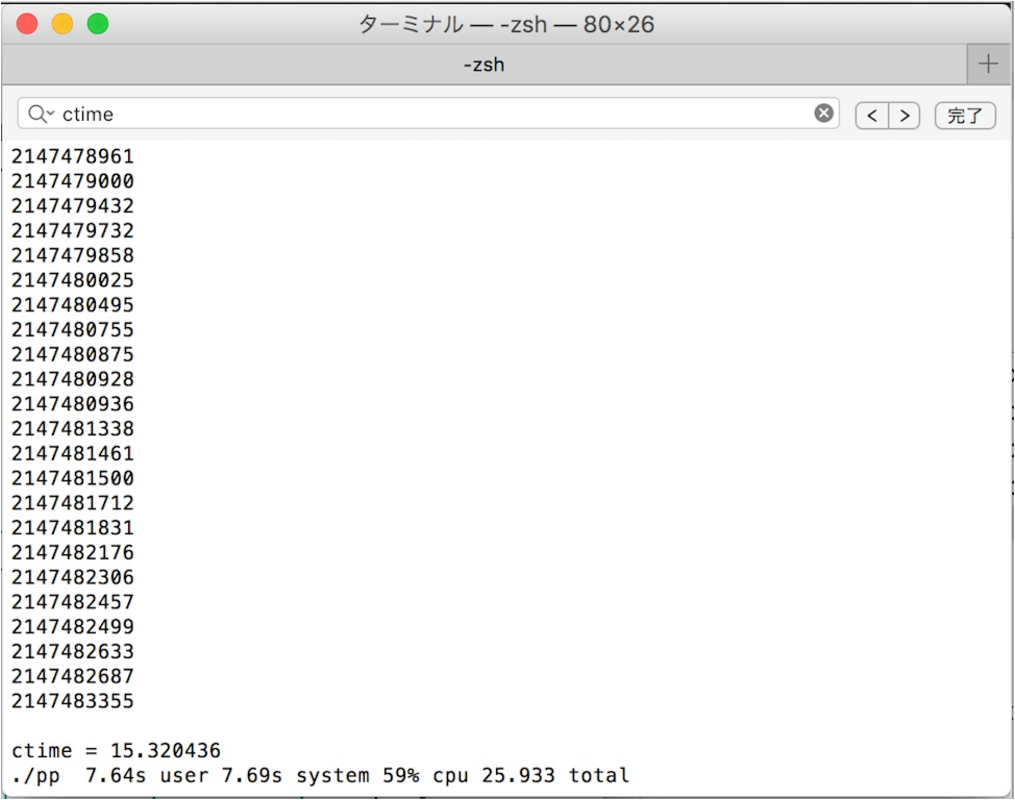
\includegraphics[width=10cm,height=7cm]{nonpp-crop.pdf}
   \caption{逐次処理のマージソートの実行結果}
   \end{center}
  \end{minipage}
 \end{tabular}
\end{figure}

\newpage
\begin{figure}[htbp]
 \begin{tabular}{c}
  \begin{minipage}{0.5\hsize}
   \begin{center}
   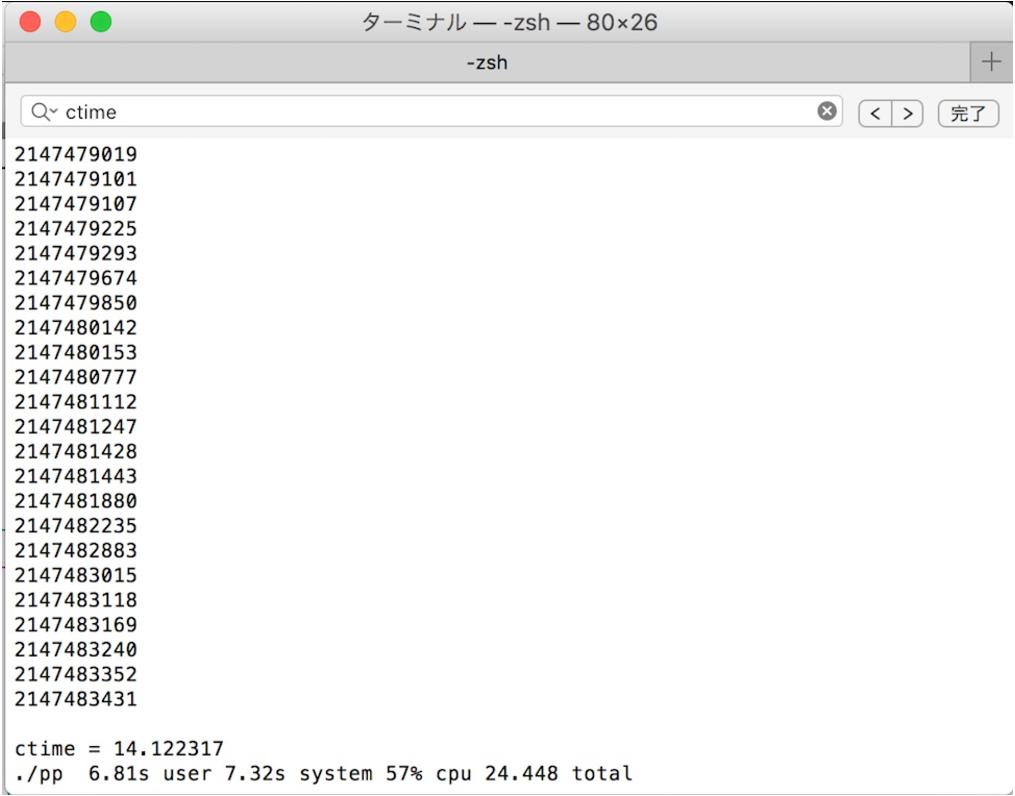
\includegraphics[width=10cm,height=7cm]{pp-crop.pdf}
   \caption{並列化したマージソートの実行結果}
   \end{center}
  \end{minipage}
 \end{tabular}
\end{figure}
並列化したマージソートの方が、若干ではあるが処理にかかる時間(totalの時間)が早くなっている。\\
 以上の実行を100万から1000万の間で行い得られた結果が以下のグラフである。(pp.mergeが並列、non-pp.mergeが逐次)
\begin{figure}[htbp]
 \begin{tabular}{c}
  \begin{minipage}{0.5\hsize}
   \begin{center}
   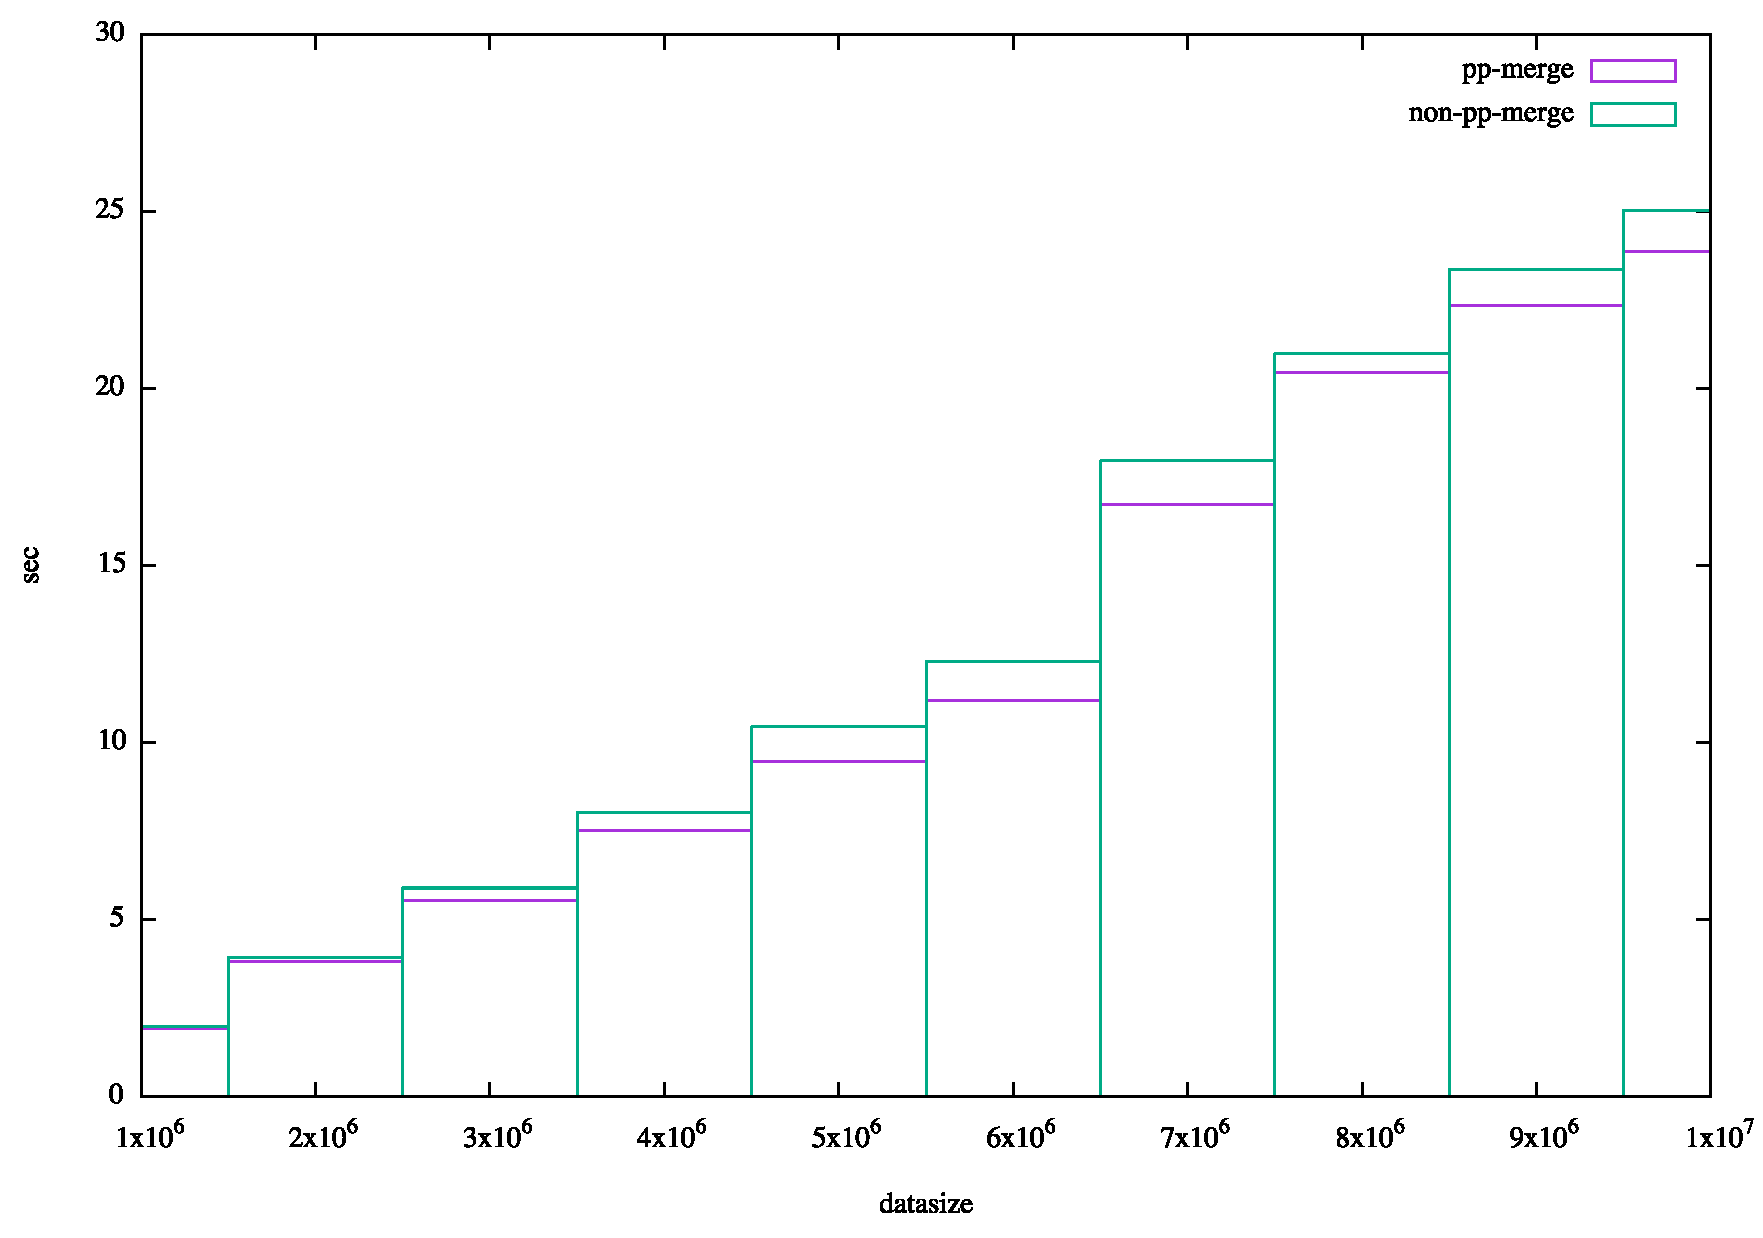
\includegraphics[width=10cm,height=7cm,angle=0]{total_graph.pdf}
   \caption{処理時間}
   \end{center}
  \end{minipage}
 \end{tabular}
\end{figure}

\newpage
\begin{figure}[htbp]
 \begin{tabular}{c}
  \begin{minipage}{0.5\hsize}
   \begin{center}
   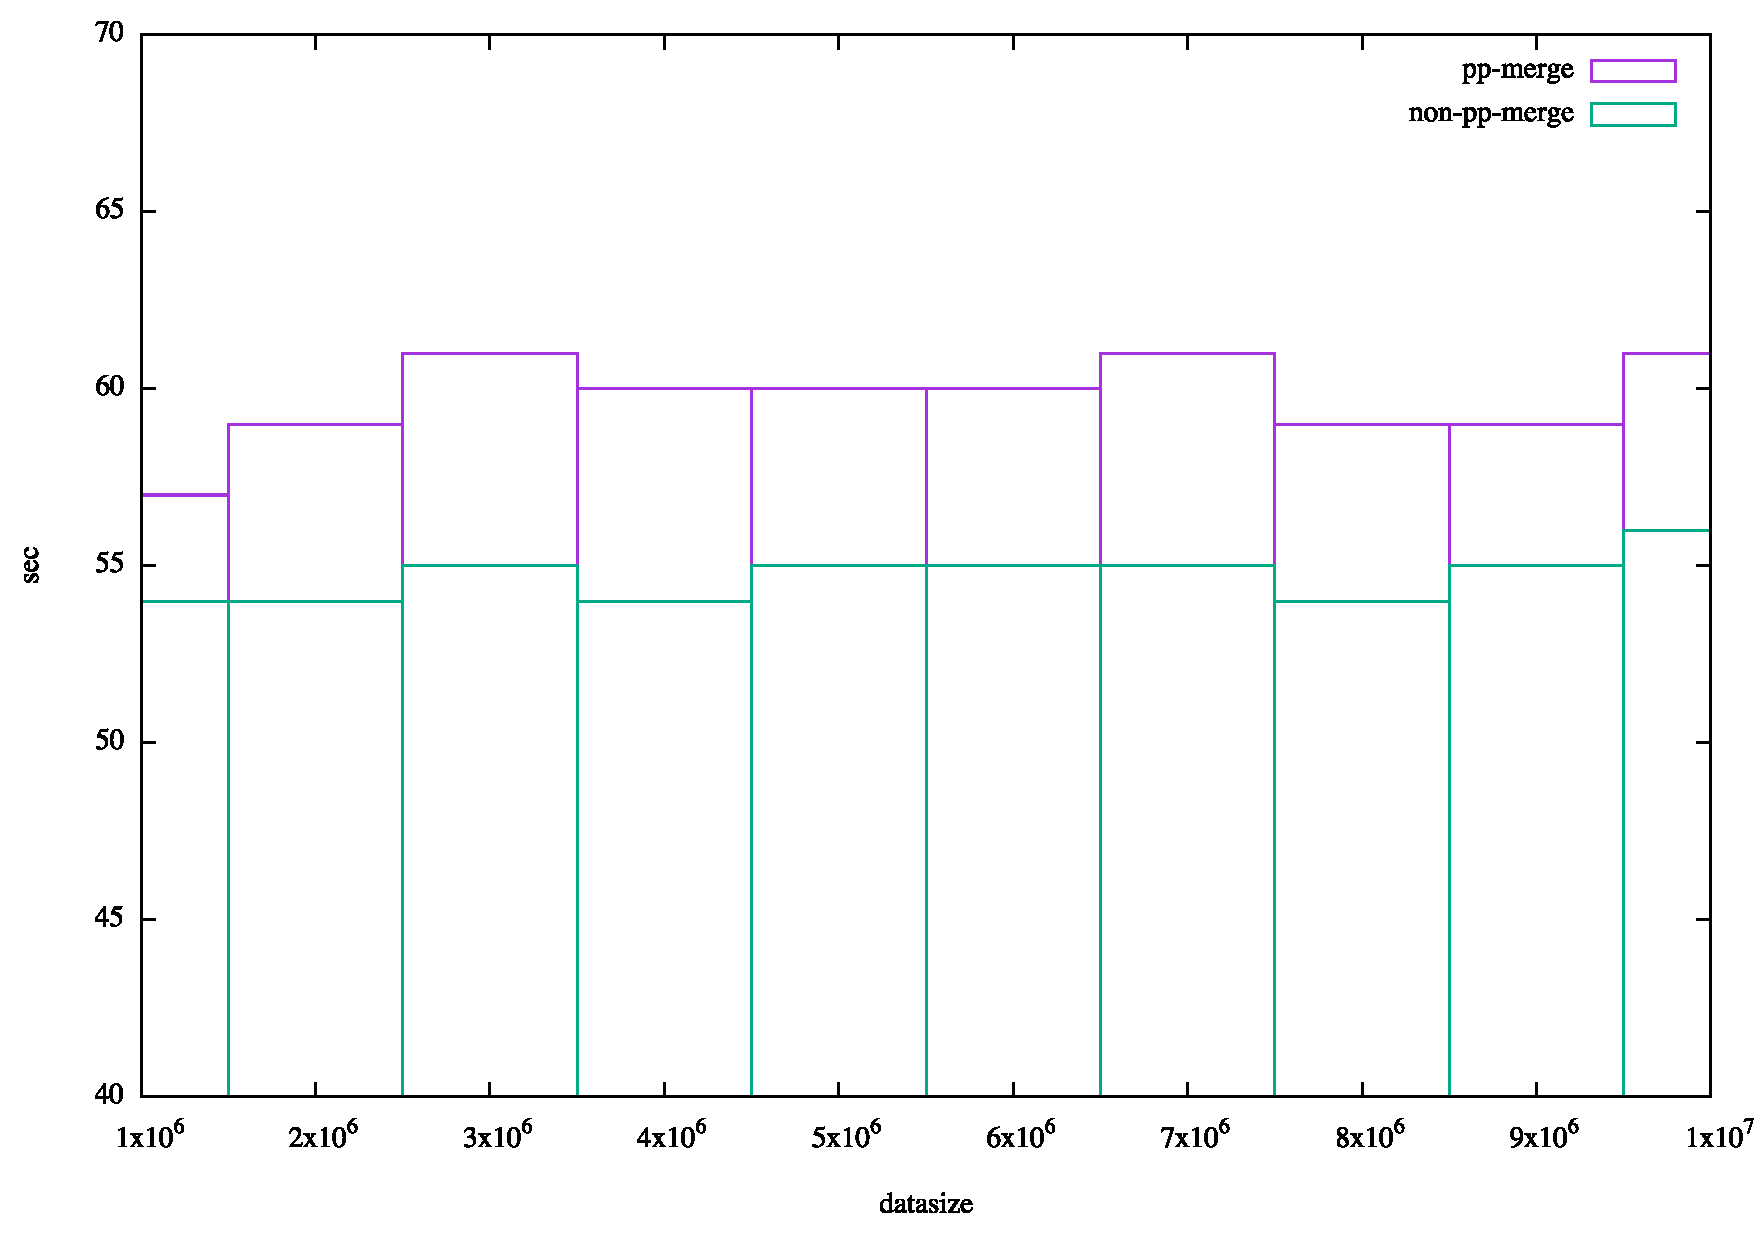
\includegraphics[width=10cm,height=7cm,angle=0]{cpu_graph.pdf}
   \caption{CPU使用率}
   \end{center}
  \end{minipage}
 \end{tabular}
\end{figure}
処理時間は、全体的に並列化した時の方が若干早くなっており、\\
 CPU使用率は、すべての実行結果で並列化した時の方が高くなっている。\\
\\
 また、以下に実際に作成したかったプログラムを添付する。\\
 (入力を受け取りランダムにシャッフルしているが、NULL文字まで受け取りシャッフルしてしまっている。)
\begin{figure}[htbp]
 \begin{tabular}{c}
  \begin{minipage}{0.5\hsize}
   \begin{center}
   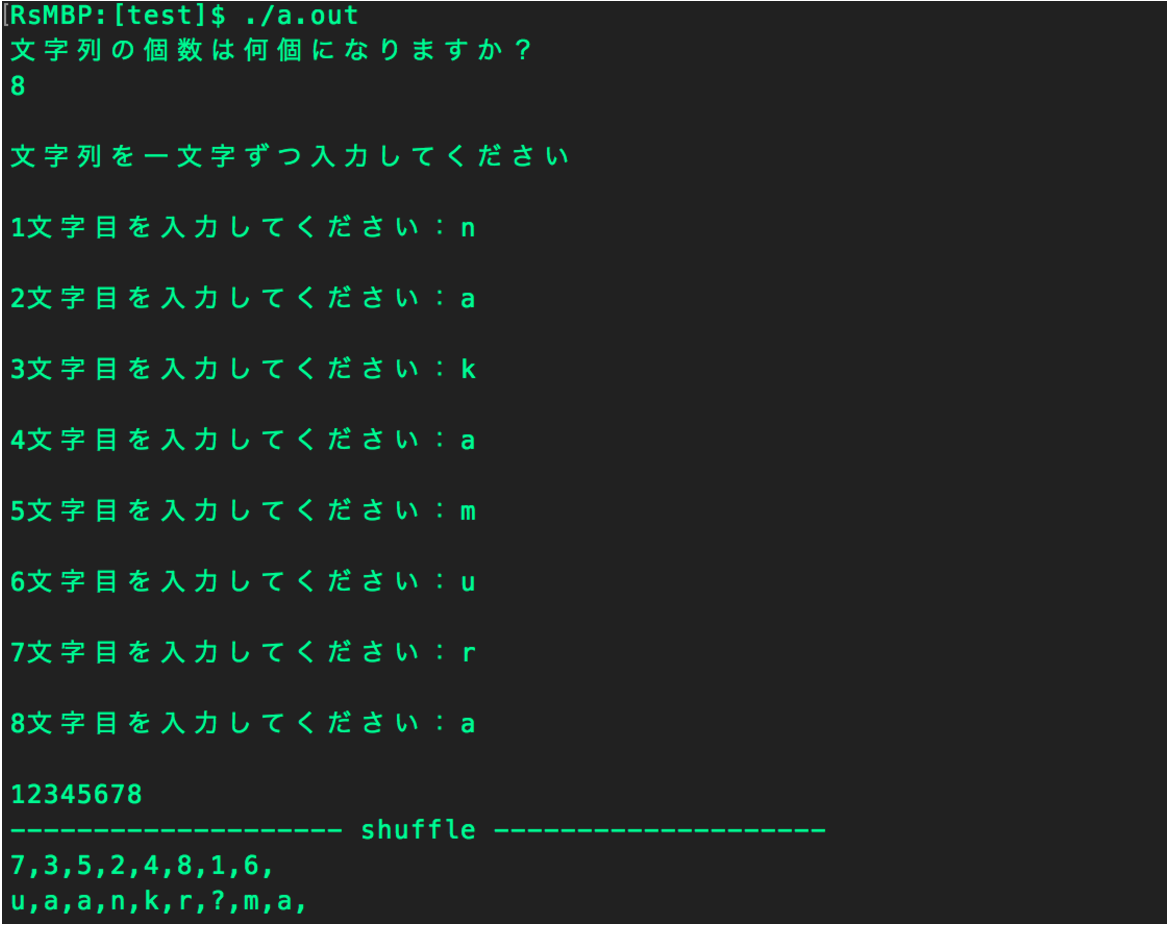
\includegraphics[width=10cm,height=7cm,angle=0]{image4-crop.pdf}
   \caption{実際に仕上げたかったプログラム}
   \end{center}
  \end{minipage}
 \end{tabular}
\end{figure}

\section*{考察}
今回初期の計画としては文字列を引数として与えてその文字列をランダムな確率でバラバラにしてソートして元の文字列に戻す、という処理を行いたかった。入力された文字列をshuffle関数というその時の時間でランダムに文字列を入れ替える関数を使って文字列をバラバラにした。しかし、C言語と文字列の相性の悪さがここで顕著に現れてきた。NULL文字の扱いや構造体へのデータの格納などと時間の関係上、実装が困難であると判断せざるを得なかった。そこで、ある大きさの数列をランダムに生成して並列化、ソートするという手法に切り替えました。またその際に比較対象として並列化していないソートを用意して比較した。\\
 実行結果はグラフの通り、全体的に処理時間は並列化した方が早く、CPU使用率は並列化すると高くなった。CPU使用率が高くなるのは、並列化処理にかかる準備(スレッドの作成など)の際にCPUをしているためだろう。また、処理時間の差が若干しか見られないのは、マージソートの処理時間が最悪でもO(n logn)であるためそもそもの処理が高速であり、並列化の効果があまり顕著に感じられないからではないかと考察した。



\end{document}